The key differentiator of our VQA model is that it is able to usefully combine image information with that extracted from a Knowledge Base, within the LSTM framework. The novelty lies in the fact that this is achieved by representing both of these disparate forms of information as text before combining them. Figure~\ref{frame} summarises how this is achieved: given an image, an attribute-based  representation $\Att(I)$ (in Section \ref{subsec:Attributes_Predictor}) is first generated and it will used as one of input sources of our VQA-LSTM model. The second input source are those captions generated in section \ref{subsec:caption_model}. Rather than inputing the generated words directly, the hidden state vector of the caption-LSTM after it has generated the last word in each caption is used to represent its content. Average-pooling is applied over the 5 hidden-state vectors, to obtain a vector representation $\Cap(I)$ for the image~$I$. The third input source is the textual knowledge which is mined from a large-scale knowledge base, the DBpedia. More details are shown in the following section.

\subsection{Relating to the Knowledge Base}

The external data source that we use here is DBpeida~\cite{auer2007dbpedia} as a source of general background information, although any such KB could equally be applied. DBpeida is a structured database of information extracted from Wikipedia. The whole DBpedia dataset describes $4.58$ million entities, of which $4.22$ million are classified in a consistent ontology. The data can be accessed using an SQL-like query language for RDF called SPARQL. Given an image and its predicted attributes, we use the top-five\footnote{We only use top-5 attributes to query the KB because, based on observation of training data, an image typically contains 5-8 attributes. We also tested with top-10, but no improvements were observed.} most strongly predicted attributes to generate DBpedia queries. There are a range of problems with DBpedia and similar, however, including the sparsity of the information, and the inconsistency of its representation. Inspecting the database shows that the `comment' field is the most generally informative about an attribute, as it contains a general text description of it.  We therefore retrieve the comment text for each query term. The KB+SPARQL combination is very general, however, and could be applied problem specific KBs, or a database of common sense information, and can even perform basic inference over RDF. Figure~\ref{img:example_rdf} shows an example of the query language and returned text.

Since the text returned by the SPARQL query is typically much longer than the captions generated in the section \ref{subsec:caption_model}, we turn to Doc2Vec \cite{le2014distributed} to extract the semantic meanings\footnote{We investigated to use an LSTM to encode the mined paragraphs, but we observed little performance improvement, despite the additional training overhead.}. Doc2Vec, also known as Paragraph Vector, is an unsupervised algorithm that learns fixed-length feature representations from variable-length pieces of texts, such as sentences, paragraphs, and documents. Le \etal \cite{le2014distributed}  proved that it can capture the semantics of paragraphs. A Doc2Vec model is trained to predict words in the document given the context words. We collect 100,000 documents from  DBpedia to train a model with vector size 500. To obtain the knowledge vector $\Know(I)$ for image $I$, we combine the 5 returned paragraphs in to a single large paragraph, before semantic features using our pre-trained Doc2Vec model.

\vspace{-10pt}
\subsection{Question-guided Knowledge Selection}
\label{subsec:selected}
We incrementally implemented a question-guided knowledge selection scheme to rule out the noise information, since we observed that some mined knowledge are not necessary for answering the given question. For example, if the question is asking about the `dog' in the image, it does not make sense to input a piece of `bird' knowledge into the model, although the image does have a `bird' inside.

Given a question $Q$ and mined $n$ knowledge paragraphs using above KB+SPARQL combination, we first use our pre-trained Doc2Vec model to extract the semantic feature $V(Q)$ of the question and the feature $V(K_i)$ for each single knowledge paragraph, where $i \in n$. Then, we find the $k$ closest knowledge paragraphs to the question based on the cosine similarity between the $V(Q)$ and $V(K_i)$. Finally, we combine the $k$ selected knowledge paragraphs in to a single one and use the Doc2Vec model to extract its semantic feature. In our experiments, we set $n=10, k=5$.

\begin{figure*}[t!]
\begin{center}
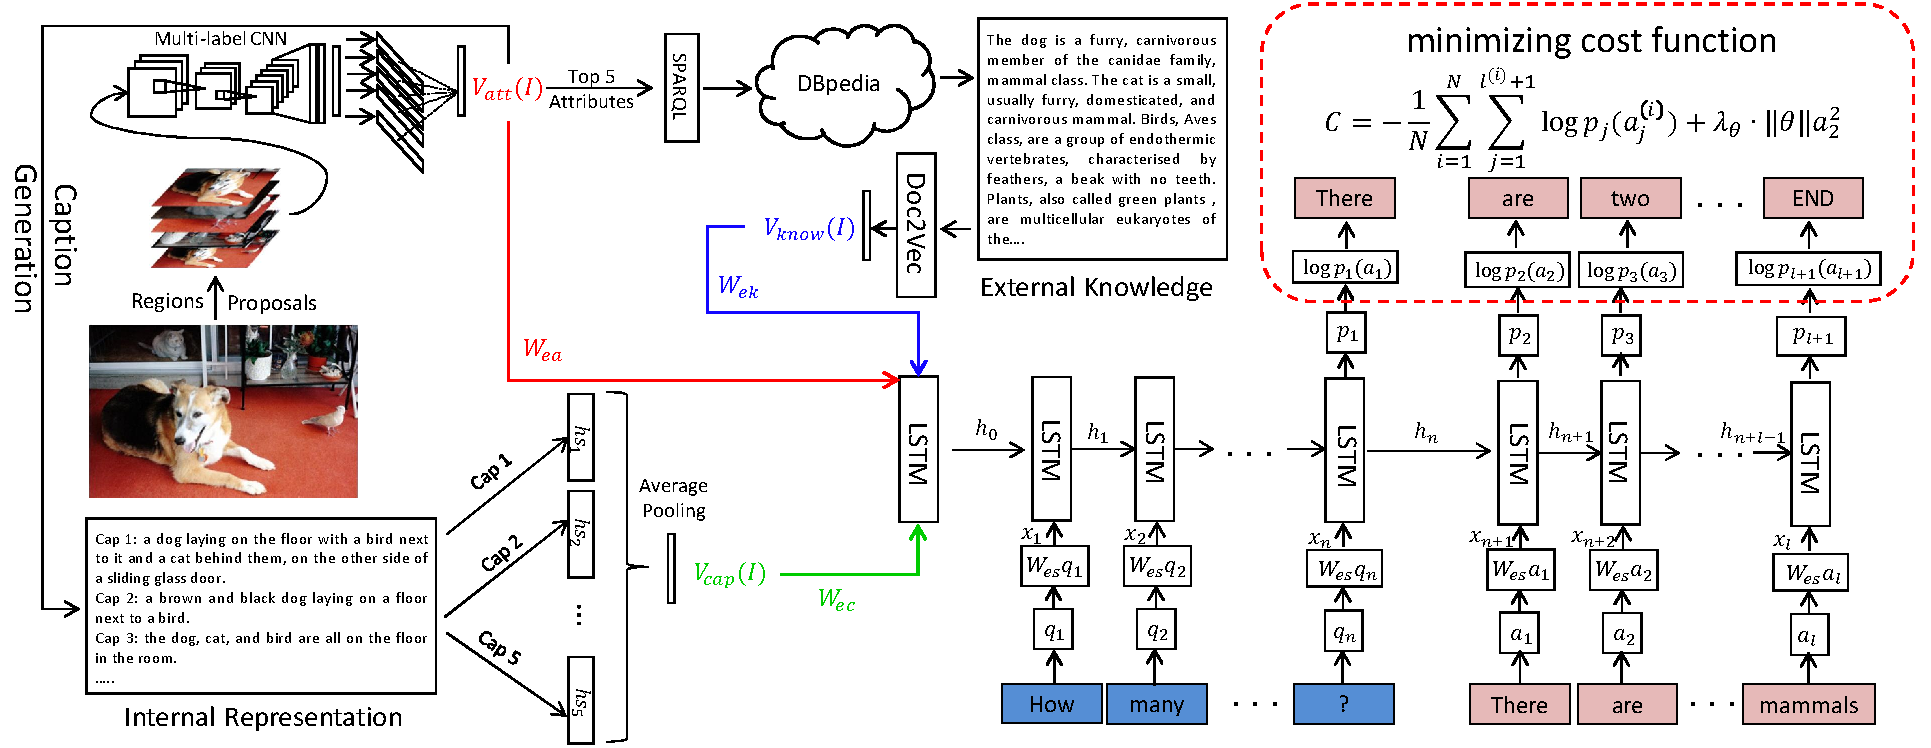
\includegraphics[width=0.95\linewidth]{img/frame_VQA.pdf}
\end{center}
\vspace{-10pt}
   \caption{Our proposed model: given an image, a CNN is first applied to produce the attribute-based representation \textcolor{red}{$\Att(I)$}. The internal textual representation is made up of image captions generated based on the image-attributes.
   %
   The hidden state of the caption-LSTM after it has generated the last word in each caption is used as its vector representation. These vectors are then aggregated as \textcolor{green}{$\Cap(I)$} with average-pooling. The external knowledge is mined from the KB and the responses are encoded by Doc2Vec, which produces a vector \textcolor{blue}{$\Know(I)$}. The 3 vectors $\mathbf{V}$ are combined into a single representation of scene content, which is input to the VQA LSTM model that interprets the question and generates an answer.
   }
   \label{frame}
   \vspace{-10pt}
\end{figure*}


\vspace{-10pt}
\subsection{An Answer Generation Model with Multiple Inputs}
We propose to train a VQA model by maximizing the probability of the correct answer given the image and question. We want our VQA model to be able to generate multiple word answers, so we formulate the answering process as a word sequence generation procedure. Let $Q=\{q_1,...,q_n\}$ represent the sequence of words in a question, and $A=\{a_1,...,a_l\}$ the answer sequence, where $n$ and $l$ are the length of question and answer, respectively. The log-likelihood of the generated answer can be written as: 
\begin{equation}
    \log p(A|I,Q)=\sum_{t=1}^l \log p(a_{t}|a_{1:t-1},I,Q)  
\end{equation}
where $p(a_t|a_{1:t-1},I,Q)$ is the probability of generating $a_t$ given image information $I$, question $Q$ and previous words $a_{1:t-1}$. We employ an encoder LSTM~\cite{hochreiter1997long} to take the semantic information from image $I$ and the question $Q$, while using a decoder LSTM to generate the answer. Weights are shared between the encoder and decoder LSTM.

\begin{figure}[t]
  \centering
  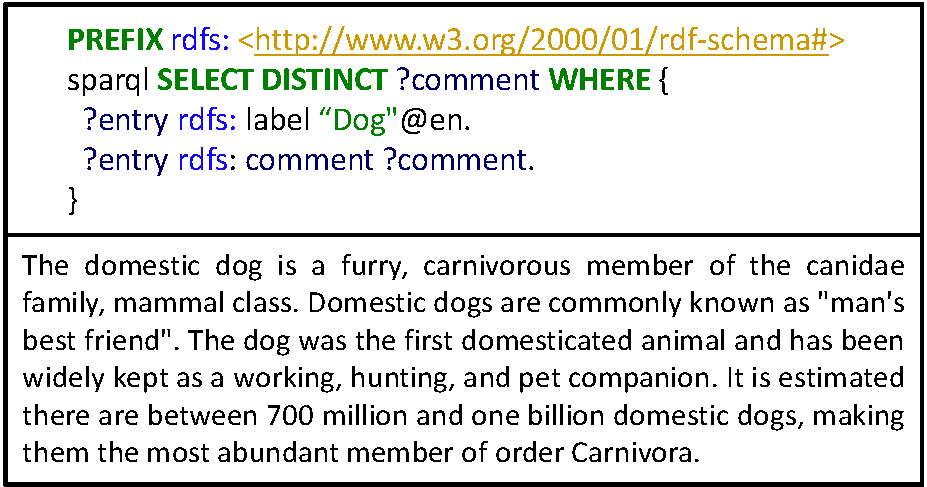
\includegraphics[width=0.9\linewidth]{img/rdf_example.pdf}
  \vspace{-3pt}
  \caption{An example of SPARQL query language for the attribute \texttt{`dog'}. The mined text-based knowledge are shown below.}
  \label{img:example_rdf}
  \vspace{-13pt}
\end{figure}

In the training phase, the question $Q$ and answer $A$ are concatenated as $\{q_1,...,q_n,a_1,...,a_l,a_{l+1}\}$, where $a_{l+1}$ is a special END token. Each word is represented as a one-hot vector of dimension equal to the size of the word dictionary. The training procedure is as follows: at time step $t=0$, we set the LSTM input: 
\begin{equation}
   x_{initial}=[ W_{ea}\Att(I), W_{ec}\Cap(I), W_{ek}\Know(I) ] 
\end{equation}
where $W_{ea}$, $W_{ec}$, $W_{ek}$ are learnable embedding weights for the vector representation of attributes, captions and external knowledge, respectively. Given the randomly initialized hidden state, the encoder LSTM feeds forward to produce  hidden state $h_{0}$ which encodes all of the input information. From $t=1$ to $t=n$, we set $x_t=W_{es}q_t$ and the hidden state $h_{t-1}$ is given by the previous step, where $W_{es}$ is the learnable word embedding weights. The decoder LSTM runs from time step $n+1$ to $l+1$. Specifically, at time step $t=n+1$, the LSTM layer takes the input $x_{n+1}=W_{es}a_1$ and the hidden state $h_{n}$ corresponding to the last word of the question, where $a_1$ is the start word of the answer. The hidden state $h_{n}$ thus encodes all available information about the image and the question. The probability distribution $p_{t+1}$ over all answer words in the vocabulary is then computed by the LSTM feed-forward process. Finally, for the final step, when $a_{l+1}$ represents the last word of the answer, the target label is set to the END token.

Our training objective is to learn parameters $W_{ea}$, $W_{ec}$, $W_{ek}$, $W_{es}$ and all the parameters in the LSTM by minimizing the following cost function:
\begin{eqnarray}
    \mathcal{C}&=&-\frac{1}{N}\sum_{i=1}^N\log p(A^{(i)}|I,Q)+\lambda_\ModParms\cdot||\ModParms||_2^2 \\
    &=&-\frac{1}{N}\sum_{i=1}^N\sum_{j=1}^{l^{(i)}+1}\log p_j(a_j^{(i)})+\lambda_\ModParms\cdot||\ModParms||_2^2
\end{eqnarray}
where $N$ is the number of training examples, and $n^{(i)}$ and $l^{(i)}$ are the length of question and answer respectively for the $i$-th training example. Let $p_t(a_t^{(i)})$ correspond to the activation of the Softmax layer in the LSTM model for the $i$-th input and $\ModParms$ represent the model parameters. Note that $\lambda_\ModParms\cdot||\ModParms||_2^2$ is a regularization term, where $\lambda_\theta=0.5\times10^{-8}$. We use Stochastic gradient Descent (SGD) with mini-batches of 100 image-QA pairs. The attributes, internal textual representation, external knowledge embedding size, word embedding size and hidden state size are all 256 in all experiments. The learning rate is set to 0.001 and clip gradients is 5. The dropout rate is set to 0.5.
